\section{Methodology}
\label{sec:methodology}

\subsection{Unsuccessful Methods}
\label{sec:methodology:unsuccessfulMethods}
Multiple extrusion methods were explored to arrive at the final methodology discussed in this paper. These are briefly included to provide context and assist future teams conducting similar research.

\subsubsection{Powder Extrusion}
While literature and industry expertise agreed that pellet-based extrusion is preferable to powder-based extrusions, powder extrusion was first tested as a means of synthesizing PLCL~\cite{RefWorks:RefID:370-einsteinisaac}.

At the time of this publication, PLCL was not commercially available in extrudable pellets. As a result, Nomisma 70/30 PLCL powder was sourced for initial extrusion work~\cite{RefWorks:RefID:387-nomisma}.

\threesubsection{Material Preparation}

Prior to extruding, the PLCL powder was dried in a vacuum oven at 45\textcelsius ~overnight based on the material manufacturer's recommendations. The Polymer Synthesis Research Facility (PSRF) at The Ohio State University was utilized for this task given their access to specialized equipment.

\threesubsection{Performing Powder Extrusion}

The powder was measured and poured into a 3Devo Filament Maker One extruder as shown in Figure~\ref{fig:methodology:extrudingPLCL:powderExtrusion}~\cite{RefWorks:RefID:393-3devo}.

\begin{figure}[h!]
        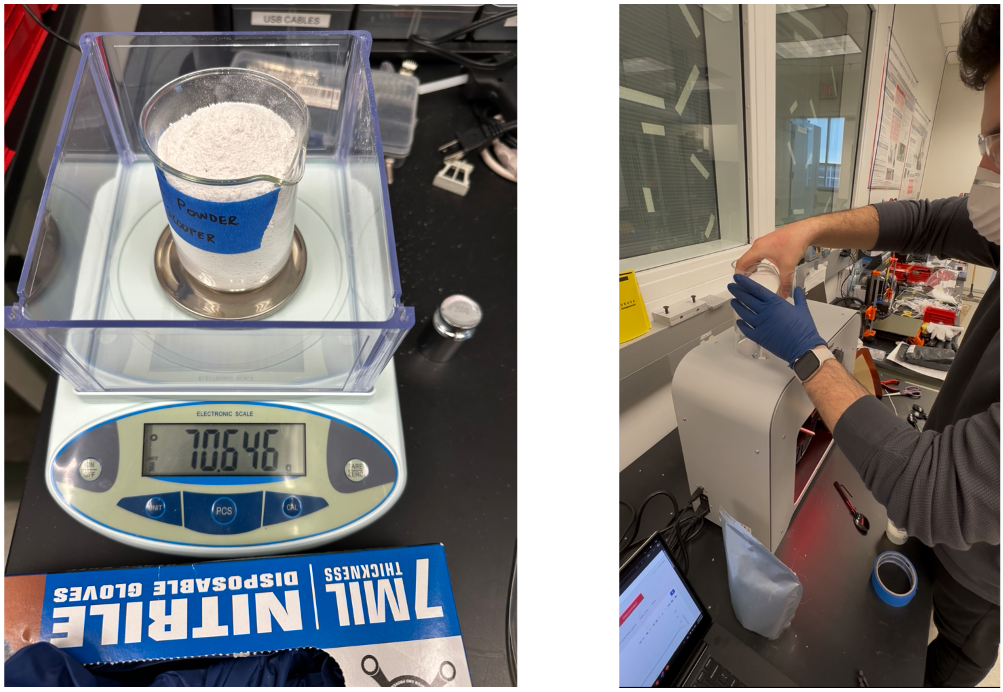
\includegraphics[width=\linewidth]{./figs/methodology/powderExtrusion/powder_extrusion.png}
        \caption{Performing PLCL powder extrusion. Measuring powder (left) and pouring into extruder (right).}
        \label{fig:methodology:extrudingPLCL:powderExtrusion}
\end{figure}

In addition to pouring the powder, a pusher inspired by the 3Devo "Devostick" was employed~\cite{RefWorks:RefID:396-3devotroubleshooting}. This is a rectangular piece of wood used to compress the material in hopes of resolving feeding issues. Using the pusher piece is shown below in Figure~\ref{fig:methodology:extrudingPLCL:devostick}.

\begin{figure}[h!]
        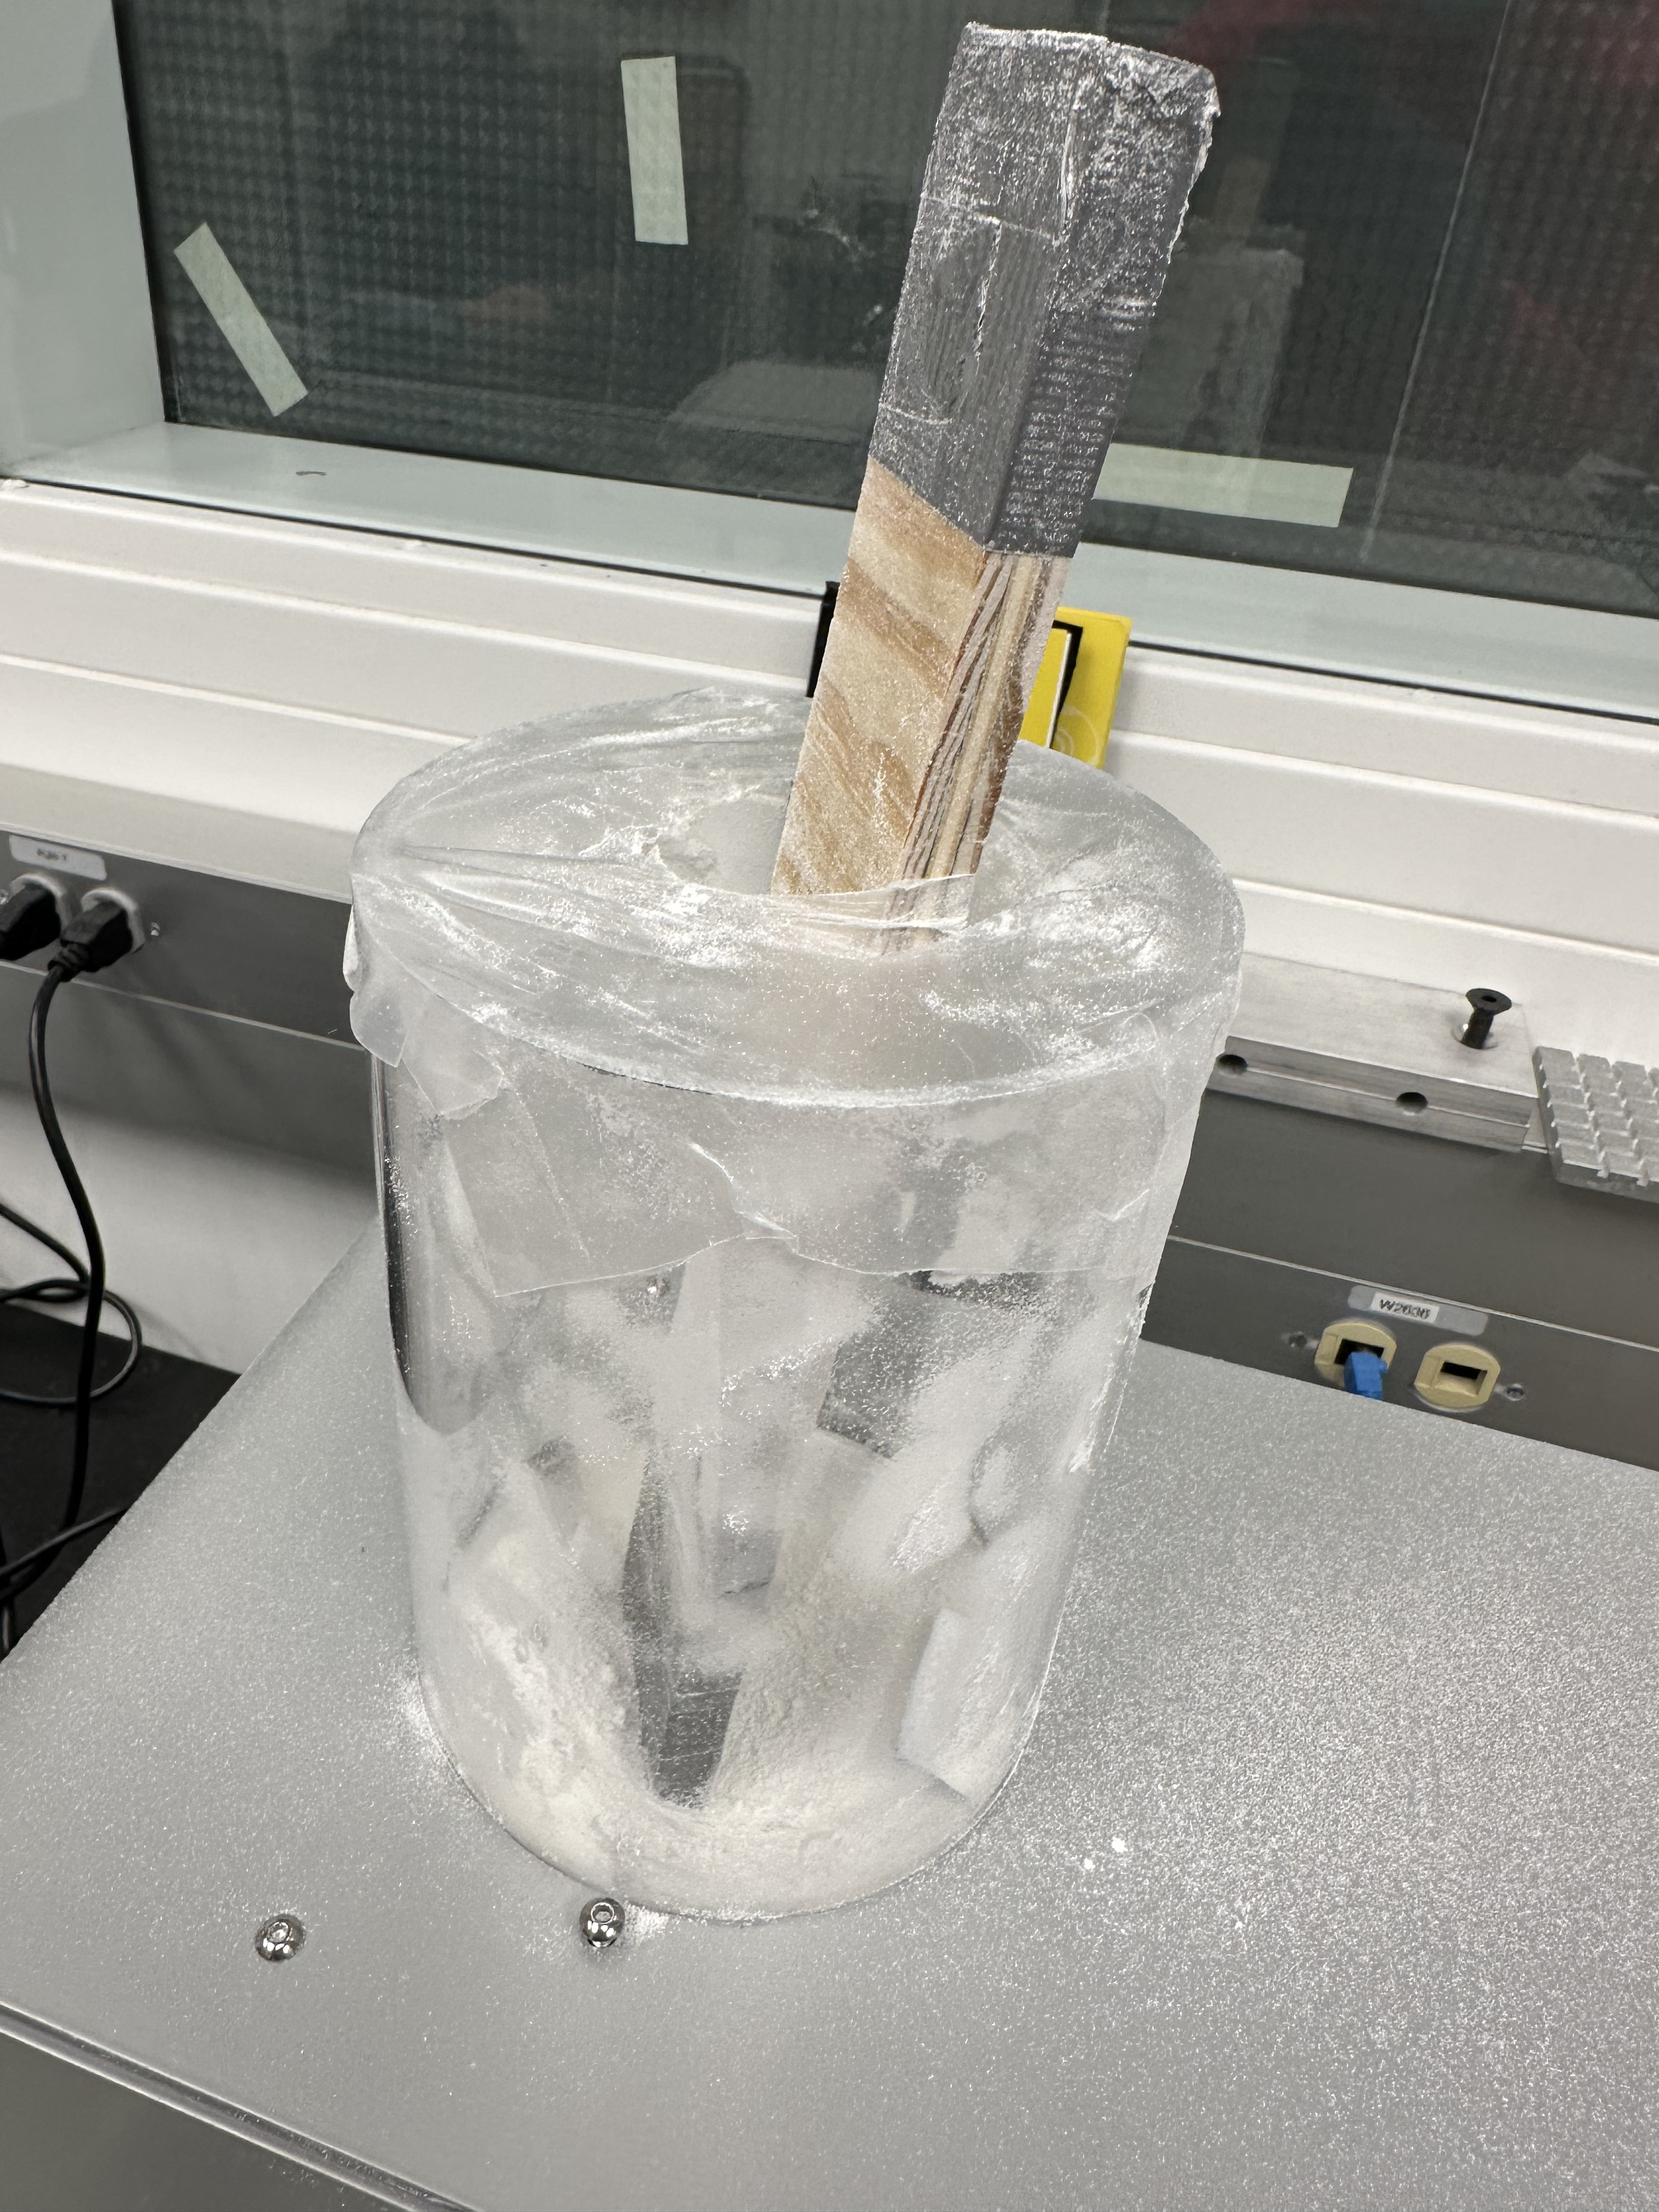
\includegraphics[width=0.5\linewidth]{./figs/methodology/powderExtrusion/devostick.png}
        \caption{Using the self-made 3Devo "Devostick".}
        \label{fig:methodology:extrudingPLCL:devostick}
\end{figure}

This extruder has four heat zones with heater 4 (H4) being closest to the hopper and heater 1 (H1) being closest to the nozzle. Heaters 4 through 1 were set to 205\textcelsius, 200\textcelsius, 195\textcelsius, and 190\textcelsius ~respectively based on 3Devo customer support recommendations. The RPM for the extruder was set to 3.5.

To achieve these temperatures, the extruder was first run at PLA presets (H4-H1: 170, 185, 190, 170 (all in \textcelsius)). Temperatures were raised to HDPE presets (190\textcelsius ~across all heat zones) and HDPE was introduced into the extruder. Finally, temperatures were raised to the PLCL extruding temperatures and the PLCL powder was introduced into the extruder. 3Devo's custom data logging software, DevoVision, was used to monitor extruder parameters and variables such as current and heater temperatures to assess extrusion success.

\threesubsection{Powder Extrusion Key Findings}

The output of the PLCL extrusion is shown below in Figure~\ref{fig:results:extrudingPLCL:powderExtrusion:filamentOutput}.

\begin{figure}[h!]
        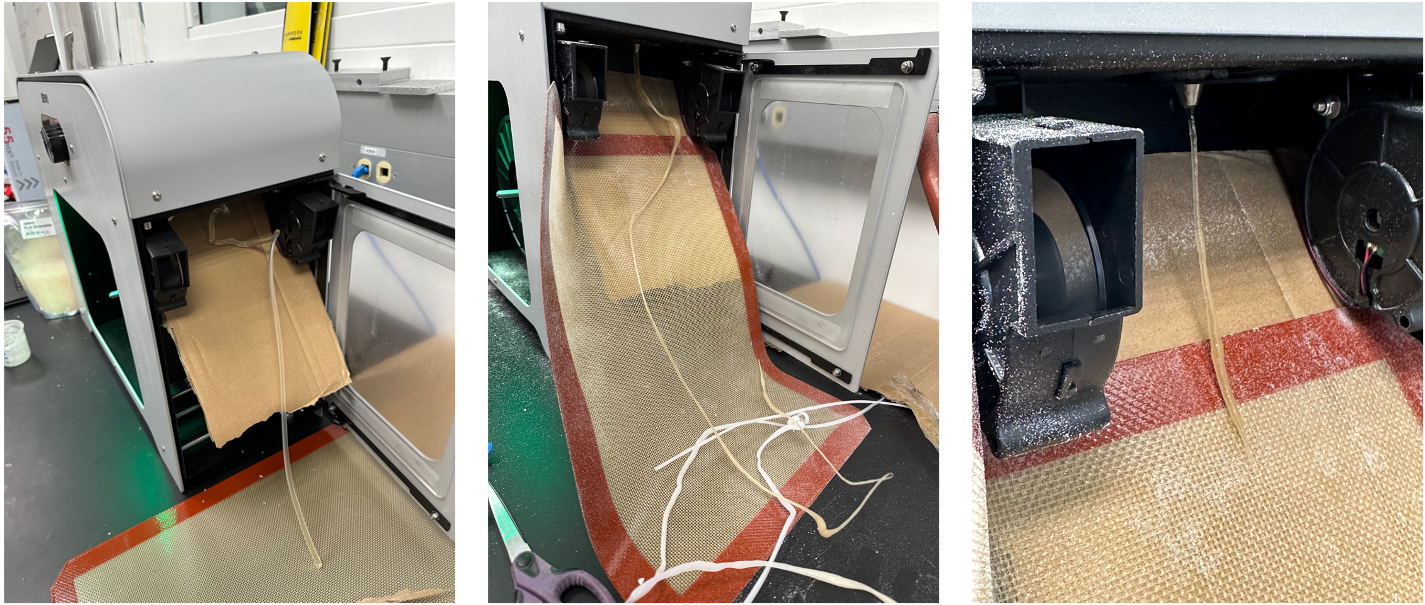
\includegraphics[width=\linewidth]{./figs/methodology/powderExtrusion/powder_filament_output.png}
        \caption{Extruder output of PLCL powder extrusion. Initial PLA output, transition from HDPE to PLCL (middle), and fully PLCL output (right).}
        \label{fig:results:extrudingPLCL:powderExtrusion:filamentOutput}
\end{figure}

The current output in $mA$ throughout this extrusion is shown below in Figure~\ref{fig:results:extrudingPLCL:powderExtrusion:currentOutput}. This was collected through DevoVision.

\begin{figure}[h!]
        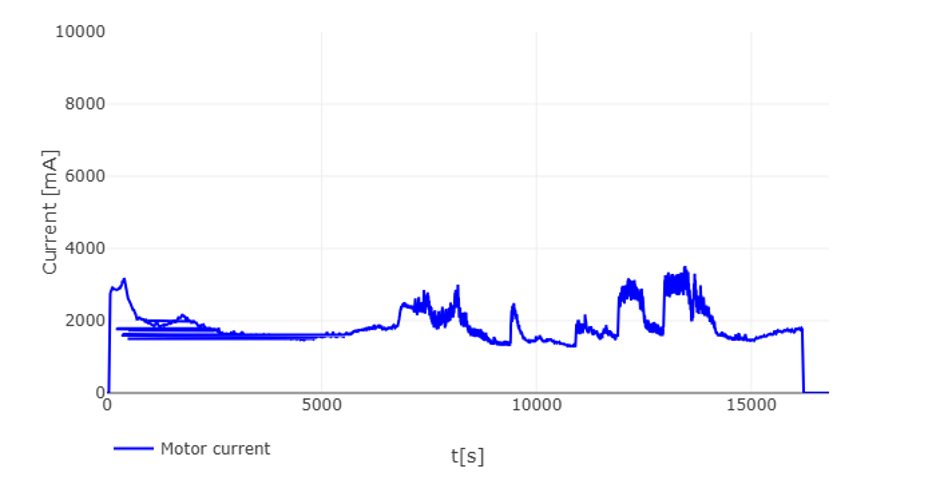
\includegraphics[width=\linewidth]{./figs/methodology/powderExtrusion/powder_current_output.png}
        \caption{Current output throughout PLCL powder extrusion.}
        \label{fig:results:extrudingPLCL:powderExtrusion:currentOutput}
\end{figure}

While the extrusion was successful in that filament was extruded, the output was inconsistent and unprintable. The filament was highly brittle and could snap easily. Adjustments to equipment, extrusion process, and material preparation were unsuccessful at addressing brittleness.

Additionally, the output was thin and experienced a variable flow rate as shown in the current spikes in Figure ~\ref{fig:results:extrudingPLCL:powderExtrusion:currentOutput}.

As a result, alternative pellet-based approaches were explored further following the unsuccessful powder-based extrusions.

\subsubsection{Pellets Sitting in Hopper}

\subsection{PLCL Synthesis}
\label{sec:methodology:plclSynthesis}

\subsubsection{Equipment Used}

\subsubsection{Combining Raw Materials}

\subsubsection{Extruding Regrind}

\subsection{Material Characterization Testing}
\label{sec:methodology:materialCharacterization}

\subsubsection{Filament Thickness}

\subsubsection{NMR Testing}